\documentclass{standalone}
\usepackage{tikz}
\usetikzlibrary{positioning}
\begin{document}
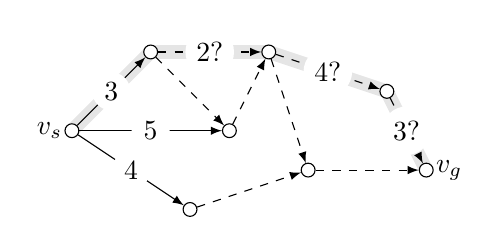
\begin{tikzpicture}

\tikzstyle{vertex}=[circle,draw=black,fill=white,inner sep=0pt,minimum size=5pt]

\coordinate (a) at (0,0);
\coordinate (b) at (2,0);
\coordinate (c) at (2.5,1);
\coordinate (d) at (1,1);
\coordinate (e) at (3,-0.5);
\coordinate (f) at (4,0.5);
\coordinate (g) at (4.5,-0.5);
\coordinate (h) at (1.5,-1);

\draw[black!10,line width=5pt,line cap=round] (a) -- (d) -- (c) -- (f) -- (g);

\node[vertex] (na) at (a) {};
\node[vertex] (nb) at (b) {};
\node[vertex] (nc) at (c) {};
\node[vertex] (nd) at (d) {};
\node[vertex] (ne) at (e) {};
\node[vertex] (nf) at (f) {};
\node[vertex] (ng) at (g) {};
\node[vertex] (nh) at (h) {};

\draw[black,->,>=latex] (na) -- (nb) node [circle,inner sep=2pt,midway,fill=white] {5};
\draw[black,->,>=latex] (na) -- (nh) node [circle,inner sep=2pt,midway,fill=white] {4};
\draw[black,->,>=latex] (na) -- (nd) node [circle,inner sep=2pt,midway,fill=white] {3};
\draw[black,->,dashed,>=latex] (nd) -- (nb);
\draw[black,->,dashed,>=latex] (nb) -- (nc);
\draw[black,->,dashed,>=latex] (nd) -- (nc) node [circle,inner sep=2pt,midway,fill=white] {2?};
\draw[black,->,dashed,>=latex] (nc) -- (ne);
\draw[black,->,dashed,>=latex] (nc) -- (nf) node [circle,inner sep=2pt,midway,fill=white] {4?};
\draw[black,->,dashed,>=latex] (nf) -- (ng) node [circle,inner sep=2pt,midway,fill=white] {3?};
\draw[black,->,dashed,>=latex] (ne) -- (ng);
\draw[black,->,dashed,>=latex] (nh) -- (ne);

\node[left=0pt of a] {$v_s$};
\node[right=0pt of g] {$v_g$};

\end{tikzpicture}%
\end{document}
